\subsection{圆和圆的位置关系}\label{subsec:czjh2-7-13}

从图 \ref{fig:czjh2-7-49} 的一些圆形部件之间的相互位置关系中可以看出,同一平面内的两个圆,可能有下面的几种位置关系:

\begin{figure}[htbp]
    \centering
    \begin{minipage}[b]{8cm}
        \centering
        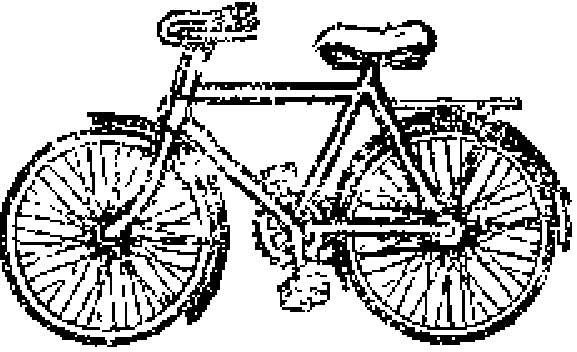
\includegraphics[width=7cm]{../pic/czjh2-ch7-49-1.png}
        \caption*{自行车}
    \end{minipage}
    \begin{minipage}[b]{6cm}
        \centering
        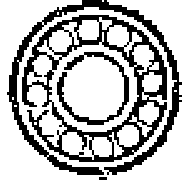
\includegraphics[width=3cm]{../pic/czjh2-ch7-49-2.png}
        \caption*{滚珠轴承}
    \end{minipage}
    \caption{}\label{fig:czjh2-7-49}
\end{figure}

(1) 两个圆没有公共点,并且每个圆上的点都在另一个圆的外部时,叫做这两个圆\zhongdian{外离}(图 \ref{fig:czjh2-7-50} 甲)。

(2) 两个圆有唯一的公共点,并且除了这个公共点以外,每个圆上的点都在另一个圆的外部时,
叫做这两个圆\zhongdian{外切}(图 \ref{fig:czjh2-7-50} 乙)。这个唯一的公共点叫做\zhongdian{切点}。


\begin{figure}[htbp]
    \centering
    \begin{minipage}[b]{4.7cm}
        \centering
        \begin{tikzpicture}[scale=.8] % 这组图中, O_1 固定不动, O_2 向 O_1 移近。所以以 O_1 为原点
    \pgfmathsetmacro{\R}{1.5}
    \pgfmathsetmacro{\r}{1.2}

    \tkzDefPoints{0/0/O_1, -3.1/0/O_2}
    \tkzDefPoint(60:\R){M}
    \tkzDefShiftPoint[O_2](60:\r){N}

    \tkzDrawCircle[thick](O_1,M)
    \tkzDrawCircle[thick](O_2,N)
    \tkzDrawSegments(O_1,M  O_2,N  O_1,O_2)
    \tkzLabelSegment[midway, left](O_1,M){$R$}
    \tkzLabelSegment[midway, left](O_2,N){$r$}
    \tkzLabelPoints[right](O_1)
    \tkzLabelPoints[left](O_2)
\end{tikzpicture}


        \caption*{甲}
    \end{minipage}
    \qquad
    \begin{minipage}[b]{4.5cm}
        \centering
        \begin{tikzpicture}[scale=.8]
    \pgfmathsetmacro{\R}{1.5}
    \pgfmathsetmacro{\r}{1.2}

    \tkzDefPoints{0/0/O_1, -2.7/0/O_2, -\R/0/T}
    \tkzDefPoint(60:\R){M}
    \tkzDefShiftPoint[O_2](60:\r){N}

    \tkzDrawCircle[thick](O_1,M)
    \tkzDrawCircle[thick](O_2,N)
    \tkzDrawSegments(O_1,M  O_2,N  O_1,O_2)
    \tkzLabelSegment[midway, left](O_1,M){$R$}
    \tkzLabelSegment[midway, left](O_2,N){$r$}
    \tkzLabelPoints[right](O_1)
    \tkzLabelPoints[left](O_2)
    \tkzLabelPoints[above=1.3em](T)
\end{tikzpicture}


        \caption*{乙}
    \end{minipage}
    \qquad
    \begin{minipage}[b]{4.5cm}
        \centering
        \begin{tikzpicture}[scale=.8]
    \pgfmathsetmacro{\R}{1.5}
    \pgfmathsetmacro{\r}{1.2}

    \tkzDefPoints{0/0/O_1, -2.3/0/O_2}
    \tkzDefPoint(60:\R){M}
    \tkzDefShiftPoint[O_2](60:\r){N}
    \tkzInterCC(O_1,M)(O_2,N)  \tkzGetPoints{B}{A}

    \tkzDrawCircle[thick](O_1,M)
    \tkzDrawCircle[thick](O_2,N)
    \tkzDrawSegments(O_1,M  O_2,N  O_1,O_2)
    \tkzLabelSegment[midway, left](O_1,M){$R$}
    \tkzLabelSegment[midway, left](O_2,N){$r$}
    \tkzLabelPoints[right](O_1)
    \tkzLabelPoints[left](O_2)
    \tkzLabelPoints[above=.5em](A)
    \tkzLabelPoints[below=.5em](B)
\end{tikzpicture}


        \caption*{丙}
    \end{minipage}
    \qquad
    \begin{minipage}[b]{4.5cm}
        \centering
        \begin{tikzpicture}[scale=.8]
    \pgfmathsetmacro{\R}{1.5}
    \pgfmathsetmacro{\r}{1.2}

    \tkzDefPoints{0/0/O_1, \r-\R/0/O_2, -\R/0/T}
    \tkzDefPoint(60:\R){M}
    \tkzDefShiftPoint[O_2](60:\r){N}

    \tkzDrawCircle[thick](O_1,M)
    \tkzDrawCircle[thick](O_2,N)
    \tkzDrawSegments(O_1,M  O_2,N  O_1,T)
    \tkzLabelSegment[pos=.7, right](O_1,M){$R$}
    \tkzLabelSegment[midway, left](O_2,N){$r$}
    \tkzLabelPoints[right](O_1)
    \tkzLabelPoints[below](O_2)
    \tkzLabelPoints[left](T)
\end{tikzpicture}


        \caption*{丁}
    \end{minipage}
    \qquad
    \begin{minipage}[b]{7cm}
        \centering
        \begin{minipage}[b]{2.8cm}
            \begin{tikzpicture}[scale=.8]
    \pgfmathsetmacro{\R}{1.5}
    \pgfmathsetmacro{\r}{1.2}

    \tkzDefPoints{0/0/O_1, \r-\R+.15/0/O_2, -\R/0/T}
    \tkzDefPoint(60:\R){M}
    \tkzDefShiftPoint[O_2](60:\r){N}

    \tkzDrawCircle[thick](O_1,M)
    \tkzDrawCircle[thick](O_2,N)
    \tkzDrawSegments(O_1,M  O_2,N  O_1,T)
    \tkzLabelSegment[pos=.4, right](O_1,M){$R$}
    \tkzLabelSegment[midway, left](O_2,N){$r$}
    \tkzLabelPoints[right](O_1)
    \tkzLabelPoints[below](O_2)
\end{tikzpicture}


        \end{minipage}
        \begin{minipage}[b]{2.8cm}
            \begin{tikzpicture}[scale=.8]
    \pgfmathsetmacro{\R}{1.5}
    \pgfmathsetmacro{\r}{1.2}

    \tkzDefPoints{0/0/O_1, 0/0/O_2} % O_1 = O_2
    \tkzDefPoint(15:\R){M}
    \tkzDefShiftPoint[O_2](60:\r){N}

    \tkzDrawCircle[thick](O_1,M)
    \tkzDrawCircle[thick](O_2,N)
    \tkzDrawSegments(O_1,M  O_2,N)
    \tkzLabelSegment[midway, below](O_1,M){$R$}
    \tkzLabelSegment[midway, left](O_2,N){$r$}
    \tkzLabelPoint[left](O_1){$O$}
\end{tikzpicture}


        \end{minipage}
        \caption*{戊}
    \end{minipage}
    \caption{}\label{fig:czjh2-7-50}
\end{figure}

(3) 两个圆有两个公共点时,叫做这两个圆\zhongdian{相交}(图 \ref{fig:czjh2-7-50} 丙)。

(4) 两个圆有唯一的公共点,并且除了这个公共点以外,一个圆上的点都在另一个圆的内部时,
叫做这两个圆\zhongdian{内切}(图 \ref{fig:czjh2-7-50} 丁)。这个唯一的公共点叫做\zhongdian{切点}。

(5) 两个圆没有公共点,并且一个圆上的点都在另一个圆的内部时,叫做这两个圆\zhongdian{内含}(图 \ref{fig:czjh2-7-50} 戊)。
两圆同心是两圆内含的一种特例。

从图 \ref{fig:czjh2-7-50} 可以看出,圆和圆的位置关系与两圆半径、圆心距的大小有关。
如果两圆的半径分别为 $R$ 和 $r$, 圆心距为 $d$,那么


\zhongdian{(1) $\bm{d > R + r} \dengjiayu$ 两圆外离;}

\zhongdian{(2) $\bm{d = R + r} \dengjiayu$ 两圆外切;}

\zhongdian{(3) $\bm{R - r < d < R + r \; (R \geqslant r)} \dengjiayu$ 两圆相交;}

\zhongdian{(4) $\bm{d = R - r \; (R > r)} \dengjiayu$ 两圆内切;}

\zhongdian{(5) $\bm{d < R - r \; (R > r)} \dengjiayu$ 两圆内含。}

在图 \ref{fig:czjh2-7-50} 中,设想 $\yuan\,O_1$ 固定不动, $\yuan\,O_2$ 从一方移近并进入 $\yuan\,O_1$,
直到圆心 $O_2$ 和 $O_1$ 重合,就可以看到上面所说的各种情况。

关于相交的两圆,有下面的定理:

\begin{dingli}[定理]
    相交两圆的连心线(经过两个圆心的直线),垂直平分两圆的公共弦。
\end{dingli}

已知:$\yuan\,O_1$ 和 $\yuan\,O_1$ 相交于点 $A$ 和 $B$ (图 \ref{fig:czjh2-7-51})。

求证: 直线 $O_1O_2$ 垂直平分线段 $AB$。

\zhengming 因为,经过圆心 $O_1$ 和 $O_2$ 的直线是 $\yuan\,O_1$ 的对称轴,又是 $\yuan\,O_2$ 的对称轴,
所以, $\yuan\,O_1$ 和 $\yuan\,O_2$ 的公共点 $A$ 的对称点在 $\yuan\,O_1$ 上,又在 $\yuan\,O_1$ 上。
这个对称点只能是两圆的另一个交点 $B$。 这样,连心线 $O_1O_2$ 就是连结对称点 $A$、$B$ 的线段的垂直平分线。

\begin{figure}[htbp]
    \centering
    \begin{minipage}[b]{5.2cm}
        \centering
        \begin{tikzpicture}[scale=.9]
    \pgfmathsetmacro{\R}{1.5}
    \pgfmathsetmacro{\r}{1.2}

    \tkzDefPoints{0/0/O_1, 2.2/0/O_2}
    \tkzDefPoint(60:\R){M}
    \tkzDefShiftPoint[O_2](60:\r){N}
    \tkzInterCC(O_1,M)(O_2,N)  \tkzGetPoints{A}{B}

    \tkzDrawCircle[thick](O_1,M)
    \tkzDrawCircle[thick](O_2,N)
    \tkzDrawPoints(O_1, O_2)
    \tkzDrawLine[add=.8 and .8](O_1,O_2)
    \tkzDrawSegments(A,B)
    \tkzLabelPoints[below](O_1)
    \tkzLabelPoints[below](O_2)
    \tkzLabelPoints[above=.5em](A)
    \tkzLabelPoints[below=.5em](B)
\end{tikzpicture}


        \caption*{} % 与下面的图水平对齐
        \caption{}\label{fig:czjh2-7-51}
    \end{minipage}
    \qquad
    \begin{minipage}[b]{10.5cm}
        \centering
        \begin{minipage}[b]{5.6cm}
            \centering
            \begin{tikzpicture}[scale=.9]
    \pgfmathsetmacro{\R}{1.5}
    \pgfmathsetmacro{\r}{1.0}

    \tkzDefPoints{0/0/O_1, \R+\r/0/O_2, \R/0/T}
    \tkzDefPoint(60:\R){M}
    \tkzDefShiftPoint[O_2](60:\r){N}

    \tkzDrawCircle[thick](O_1,M)
    \tkzDrawCircle[thick](O_2,N)
    \tkzDrawPoints(O_1, O_2)
    \tkzDrawLine[add=.7 and .5](O_1,O_2)
    \tkzLabelPoints[below](O_1)
    \tkzLabelPoints[below](O_2)
    \tkzLabelPoints[left, yshift=.5em](T)
\end{tikzpicture}


            \caption*{甲}
        \end{minipage}
        \begin{minipage}[b]{4cm}
            \centering
            \begin{tikzpicture}[scale=.9]
    \pgfmathsetmacro{\R}{1.5}
    \pgfmathsetmacro{\r}{1.0}

    \tkzDefPoints{0/0/O_1, \r-\R/0/O_2, -\R/0/T}
    \tkzDefPoint(60:\R){M}
    \tkzDefShiftPoint[O_2](60:\r){N}

    \tkzDrawCircle[thick](O_1,M)
    \tkzDrawCircle[thick](O_2,N)
    \tkzDrawPoints(O_1, O_2)
    \tkzDrawLine[add=3.5 and 3](O_1,O_2)
    \tkzLabelPoints[below, xshift=.2em](O_1)
    \tkzLabelPoints[below, xshift=-.2em](O_2)
    \tkzLabelPoints[left, yshift=.5em](T)
\end{tikzpicture}


            \caption*{乙}
        \end{minipage}
        \caption{}\label{fig:czjh2-7-52}
    \end{minipage}
\end{figure}


关于相切的两圆,有下面的定理:

\begin{dingli}[定理]
    相切两圆的连心线,经过切点。
\end{dingli}

已知: $\yuan\,O_1$ 和 $\yuan\,O_2$ 相切于点 $T$(图 \ref{fig:czjh2-7-52})。

求证: 连心线 $O_1O_2$ 经过切点 $T$。

\zhengming 用反证法。

假设 $O_1O_2$ 不经过 $\yuan\,O_1$ 和 $\yuan\,O_2$ 的切点 $T$ (即点 $T$ 不在 $O_1O_2$ 上),
那么,点 $T$ 关于 $O_1O_2$ 的对称点 $T'$ 也不在 $O_1O_2$ 上。
由于直线 $O_1O_2$ 是 $\yuan\,O_1$ 的对称轴,又是 $\yuan\,O_2$ 的对称轴,
并且点 $T$ 是 $\yuan\,O_1$ 和 $\yuan\,O_2$ 的公共点,
所以点 $T$ 的对称点 $T'$ 也是 $\yuan\,O_1$ 和 $\yuan\,O_1$ 的公共点。
这和题设 $\yuan\,O_1$ 和 $\yuan\,O_2$ 相切相矛盾,因此假设不能成立。
连心线 $O_1O_2$ 经过切点 $T$。


\liti[0] 已知:两个等圆 $\yuan\,O_1$ 和 $\yuan\,O_2$ 相交于 $A$、$B$ 两点,
$\yuan\,O_1$ 经过点 $O_2$(图 \ref{fig:czjh2-7-53})。求 $\angle O_1AB$ 的度数。

\jie $\because$ \quad $\yuan\,O_1$ 经过点 $O_2$, $\yuan\,O_1$、$\yuan\,O_2$ 是等圆,

$\therefore$ \quad $O_1A = O_1O_2 = O_2A$。

$\therefore$ \quad $\angle O_1AO_2 = 60^\circ$。

又 $\because$ \quad $AB \perp O_1O_2$,

$\therefore$ \quad $\angle O_1AB = 30^\circ$。


\begin{figure}[htbp]
    \centering
    \begin{minipage}[b]{5.2cm}
        \centering
        \begin{tikzpicture}[scale=.9]
    \pgfmathsetmacro{\R}{1.5}

    \tkzDefPoints{0/0/O_1, \R/0/O_2}
    \tkzInterCC[R](O_1,\R)(O_2,\R)  \tkzGetPoints{A}{B}

    \tkzDrawCircle[thick](O_1,A)
    \tkzDrawCircle[thick](O_2,A)
    \tkzDrawPoints(O_1, O_2)
    \tkzDrawSegments(O_1,O_2  A,B  O_1,A  O_2,A)
    \tkzLabelPoints[left](O_1)
    \tkzLabelPoints[right](O_2)
    \tkzLabelPoints[above=.2em](A)
    \tkzLabelPoints[below=.2em](B)
\end{tikzpicture}


        \caption{}\label{fig:czjh2-7-53}
    \end{minipage}
    \qquad
    \begin{minipage}[b]{10.5cm}
        \centering
        \begin{minipage}[b]{5.6cm}
            \centering
            \begin{tikzpicture}[scale=.9]
    \pgfmathsetmacro{\R}{1.5}
    \pgfmathsetmacro{\r}{1.0}

    \tkzDefPoints{0/0/O_1, \R+\r/0/O_2, \r/0/T}
    \tkzDefPoint(120:\r){A}
    \tkzInterLC[common=T](A,T)(O_2,T)  \tkzGetFirstPoint{B}

    \tkzDrawCircle[thick](O_1,T)
    \tkzDrawCircle[thick](O_2,T)
    \tkzDrawPoints(O_1, O_2)
    \tkzDrawSegments(O_1,A  O_2,B  A,B)
    \tkzLabelPoints[below](O_1)
    \tkzLabelPoints[right](O_2)
    \tkzLabelPoints[above](A)
    \tkzLabelPoints[below](B)
    \tkzLabelPoints[right, yshift=.5em](T)
\end{tikzpicture}


        \end{minipage}
        \begin{minipage}[b]{4cm}
            \centering
            \begin{tikzpicture}[scale=.9]
    \pgfmathsetmacro{\R}{1.5}
    \pgfmathsetmacro{\r}{1.0}

    \tkzDefPoints{0/0/O_1, \R-\r/0/O_2, -\r/0/T}
    \tkzDefPoint(60:\r){A}
    \tkzInterLC[common=T](A,T)(O_2,T)  \tkzGetFirstPoint{B}

    \tkzDrawCircle[thick](O_1,T)
    \tkzDrawCircle[thick](O_2,T)
    \tkzDrawPoints(O_1, O_2)
    \tkzDrawSegments(O_1,A  O_2,B  T,B)
    \tkzLabelPoints[below, xshift=-.5em](O_1)
    \tkzLabelPoints[below](O_2)
    \tkzLabelPoints[above, xshift=-.2em](A)
    \tkzLabelPoints[above right](B)
    \tkzLabelPoints[left](T)
\end{tikzpicture}


        \end{minipage}
        \caption*{(第 4 题)}
    \end{minipage}
\end{figure}



\begin{lianxi}

\xiaoti{$\yuan\,O_1$ 和 $\yuan\,O_2$ 的半径分别为 3 厘米和 4 厘米,设}
\begin{xiaoxiaotis}

    \begin{tblr}{columns={12em, colsep=0pt}}
        \xxt{$O_1O_2 = 8$ 厘米;} & \xxt{$O_1O_2 =   7$ 厘米;} & \xxt{$O_1O_2 = 5$ 厘米;} \\
        \xxt{$O_1O_2 = 1$ 厘米;} & \xxt{$O_1O_2 = 0.5$ 厘米;} & \xxt{$O_1$ 和 $O_2$ 重合。}
    \end{tblr}

    \quad $\yuan\,O_1$ 和 $\yuan\,O_2$ 的位置关系怎样?
\end{xiaoxiaotis}


\xiaoti{三角形的三边长分别力 4 厘米、5 厘米、6厘米,以各顶点为圆心的三个圆两两外切。
    求各圆的半径。如果三边长分别为 $a$、$b$、$c$ 呢?
}

\xiaoti{已知: $\yuan\,O_1$ 和 $\yuan\,O_2$ 相交于点 $C$ 和 $D$, $O_2O_1$ 的延长线和 $\yuan\,O_1$ 相交于点 $A$,
    $AC$、$AD$ 分别和 $\yuan\,O_2$ 相交于点 $E$、$F$。 求证: $CE = DF$。
}

\xiaoti{已知:$\yuan\,O_1$ 和 $\yuan\,O_2$ 相切于点 $T$, 经过切点 $T$ 的直线与 $\yuan\,O_1$ 和 $\yuan\,O_2$
    分别相交于另一点 $A$ 和 $B$。求证: $O_1A \pingxing O_2B$。
}

\end{lianxi}

